\documentclass[12pt,conference,compsocconf]{IEEEtran}
\usepackage{float}
\usepackage{hyperref}
\usepackage{graphicx}	% For figure environment
\usepackage{url}
\usepackage{xcolor}
\hypersetup{
    colorlinks,
    linkcolor={red!50!black},
    citecolor={blue!50!black},
    urlcolor={blue!80!black}
}
\usepackage{times}
\usepackage{tikz}
\usepackage{amsmath}
\usepackage{verbatim}
\usepackage{subfig}
\usepackage{amsthm}
\usetikzlibrary{arrows,shapes}
\newcommand\norm[1]{\left\lVert#1\right\rVert}
\newcommand{\E}{{\rm I\kern-.3em E}}

\newtheorem{innercustomgeneric}{\customgenericname}
\providecommand{\customgenericname}{}
\newcommand{\newcustomtheorem}[2]{%
  \newenvironment{#1}[1]
  {%
   \renewcommand\customgenericname{#2}%
   \renewcommand\theinnercustomgeneric{##1}%
   \innercustomgeneric
  }
  {\endinnercustomgeneric}
}

\newcustomtheorem{customthm}{Theorem}
\newcustomtheorem{customlemma}{Lemma}
\usepackage{setspace}
\setstretch{1.05}

\begin{document}
\renewcommand{\arraystretch}{1.2}

\title{Complexity analysis for AdaRBFGS: a primitive for methods between first and second order}

\author{
  Joel Castellon\\
  \textit{Supervisor:} Sebastian Stich\\
  \vspace{4mm}
  \textit{Machine Learning and Optimization Laboratory, IC School, EPFL}\\
}


\maketitle

\section{Introduction}
Matrix inversion algorithms are a fundamental sub-routine in optimization methods. Such sub-routines play an important role in the trade-off between incorporating surface information and time/memory efficiency. Which is particularly important in second order methods. Perhaps, the most well-known example is Newton's method where we are required to calculate the inverse of the Hessian (at each step) in order to incorporate second-order curvature information. While Newton's method has an excellent convergence rate (e.g. quadratic), the computational burden of calculating the inverse Hessian or even storing it becomes in-adequate for many applications.
The motivation for this work comes from studying a primitive proposed by Gower et al. in \cite{Gower1}. In Gower's work, the adaRBFGS method is proposed in an heuristic manner and stems from a more general setting that has solid theoretical ground. The authors compare, empirically, adaRBFGS against other baselines for inverting positive definite matrices and adaRBFGS outperforms these by orders of magnitude. Yet, there is still little understanding of the convergence properties of the rate for adaRBFGS as well as other more specific properties (such as dependence on the dimension of the sketch matrix, see \ref{sect:sketchdim}). Such fine grained analysis of the rate for adaRBFGS is the subject of this work and also a suggested direction for further reasearch by Gower et al. in \cite{Gower1}.

\section{Outline}
We start this report by describing the general framework that is at the origin of adaRBFGS in Section \ref{sect:rbfgs} as background. The proposed method by Gower et al. is interesting, first, because of the generalization (see Section \ref{sect:framework}) and connexion this framework makes with previously well known family of methods such as quasi-newton and simultaneous Kaczmarz just to name a few. Next, we mention, in Section \ref{sect:propertiesRBFGS}, some results and properties of adaRBFGS that will be useful for our complexity analysis. We will, then, show our results with respect to the rate complexity (Section \ref{sect:results}) of the rate via numerical experiments and theoretical justification. Finally, we make suggestions for future research and open problems we encountered in Section \ref{sect:conclusion}.

\section{RBFGS}\label{sect:rbfgs}
AdaRBFGS emerges from a framework proposed by Gower et al. in \cite{Gower1,Gower2}. The idea is to generalize quasi-newton (qN) updates, which are the primitives (matrix updates for approximating the inverse Hessian) in qN-methods. For example, take the following unconstrained optimization problem (with $f$ smooth and convex).
$\text{min}_{x \in R^n} f(x)$. The quasi-newton iteration being, $x_{k+1}=x_k-\alpha_kB_k^{-1}\nabla f(x_k)$. Now, any quasi-newton matrix $B_k$ (approximation of the Hessian) must satisfy the following constraint. $B_{k+1}(x_{k+1}-x_k)=\nabla f(x_k)-\nabla f(x_k)$. This last expression is normally referred as the \textit{secant equations}.

\subsection{General setting and geometric interpretation}\label{sect:framework}
The first idea of Gower et al. in \cite{Gower1,Gower2} is to reduce the dimension of the system for the constraints (e.g. the secant equations) while maintaining low rank updates to matrices that aim to approximate the inverse Hessian. AdaRBFGS as developed in \cite{Gower1} only considers the following version of the unconstrained optimization problem $f(x)=\frac{1}{2}x^TAx -b^Tx + c$.  Therefore, we have $A^{-1}$ as our target inverse Hessian, and the sequence of iterates to approximate $A^{-1}$ (yet the authors claim it can be adapted to approximate arbitrary matrices) are given by: 
$ X_{k+1} = \text{argmin}_{X \in R^{n\times n}} \{\frac{1}{2}\norm{X-X_k}_{F(W^{-1})}^2: S^TAX=S^T\}$ ($W$ being a parameter of the algorithm discussed later). Where $S \in R^{n\times q}$ and $q<<n$. We call $S$ the sketch matrix that will reduce the dimension of the system of equations. In its general form, $S$ can be considered a random matrix, we draw $S$ either from a fixed or varying distribution (see Section \ref{sect:adadef}). Such reduction in complexity for the constraints is, of course, at the expense of introducing many false solutions which is why we aim to take small rank updates. Gower et al. call this first formulation for the $X_k$ updates the \textit{sketch-and-approximate} point of view. Note that the sketch and project rule is a convex quadratic problem with affine constraints. Therefore, strong duality holds and the following dual update rule can be derived (see \cite{Gower1}) $X_{k+1} = \text{argmin}_{X,Y} \{\frac{1}{2}\norm{X-A^{-1}}_{F(W^{-1})}^2: X=X_k + WA^TSY^T\}$. This last expression is referred to as the \textit{constraint and approximate} point of view. There are two interesting points about this dual formulation. First, the latter type of update corresponds to the \textit{Approximate Inverse Preconditioning (AIP)} family of methods, while the former kind of update corresponds to qN updates. Then, this framework shows a previously unknown connection between qN and AIP methods. The second important point about the constrain-and-approximate rule is a geometrical interpretation which gives a more intuitive understanding of what the method does. What the constrain-and-approximate update rule says is that at each iterate $X_k$ we draw a random hyperplane crossing such point (over the distribution of $S$). Next, take the orthogonal projection of the target $A^{-1}$ in such random hyperplane as the iterate. Hence, the algorithm consists of drawing random hyperplanes crossing the iterates and projecting the objective which is $A^{-1}$.
\subsection{Adaptive RBFGS}\label{sect:adadef}
In the framework described above there are three main parameters. Namely, the distribution of random matrices $\mathcal{D}$ where $S\sim \mathcal{D}$, the weights matrix $W$ and assumptions on $A$ (e.g. symmetric or  positive definite). It turns out that most well-known quasi newton methods can be obtained by varying these these three parameters (see \cite{Gower1} for a full description). The most relevant result, for us, in this category is obtaining the Broyden-Fletcher-Goldfarb-Shanno (BFGS) by setting $W=A^{-1}$, $S$ as a deterministic vector and $A$ semi positive definite. The next step is to let $S$ be a random matrix from a fixed distribution for which we obtain RBFGS. RBFGS is a randomized block variant of the BFGS method as it can be seen as taking a block of qN-directions per iteration..\\
Next, we outline the intuition for adaRBFGS as derived in \cite{Gower1}. First, the main convergence result in \cite{Gower1} is Thm. 6.2 which outlines a rate (see Section \ref{sect:results}) in expected norm of the error. We assume that the sketch matrix sampled at each iteration $S_i$ comes from a bigger matrix (its support) which we call $\mathcal{S}$ (conditions on Section \ref{sect:propertiesRBFGS}). In section 7.1 of \cite{Gower1} the problem of determining optimal sampling probabilities is formulated as a semi definite program. Solving such SDP, however, can be even costlier than inverting $A$ itself as we iterate (support given by experiments by the authors in \cite{Gower1}). Nonetheless, the formula for the optimal probabilities obtained by the SDP (formula (62) in \cite{Gower1}) is insightful in the sense that it suggests that optimal sampling is its dependence on $A^{-1}$. However, since we do not have $A^{-1}$ we can use $X_k$ as a proxy. This is, in fact, the intuition behind the heuristic which states that sampling gets better (this being in close relation to the rate, see \ref{sect:results}) as the estimate $X_k$ is closer to the target $A^{-1}$. Now, in order to get a specific form for the support $\mathcal{S}$, an upper bound for the rate is derived in \cite{Gower2}. Such upper bound is optimal by setting $\mathcal{S}=A^{-T}W^{-1/2}=A^{-1/2}$. This means that if $X_k$ approximates $A^{-1}$ then we should sample $S_i$ (the sketch) at each iteration from the Cholesky factor $L_k$ (where $L_kL_k^T=X^k$). In fact an update rule that uses only these factors was derived in \cite{Gratton} in the context of limited memory preconditioners for BFGS. This latter update form is the one adaRBFGS uses in \cite{Gower1}\\
Next, we present two variants for the varying distribution where $S$ is sampled from (e.g. $\mathcal{D}_k$). A first such distribution is the \textit{adaRBFGS gauss} (baseline results in Fig. \ref{fig:comparison}). In adaRBFGS gauss we set $S_i=X_kG$ where $G \in R^{n\times n}$ is a random matrix of standard gaussian i.i.d entries.\\
The second variant of adaRBFGS we present is the \textit{adaRBFGS col}. This version consists of sampling $S$ as a column sub-matrix $S_i$ from $L_k=[S_1\ldots S_r]$ (where $L_kL_k^T=X_k$) with convenient probabilities $p_i$ (as defined in Section \ref{sect:convsampling}. More formally, $S=L_kI{:C_i}=S_i$ where $C_i$ is the index set corresponding to column sub-matrix $S_i$.

\subsection{Adaptive RBFGS as a primitive}\label{sect:primitive}
The RBFGS update rule (which is the same for adaRBFGS but with varying $\mathcal{D}$, see Section \ref{sect:propertiesRBFGS}) has a well-known form in the BFGS literature, and a consequence of this form is that it can be composed in a larger setting to get methods with well-known properties in the quasi Newton family. A concrete example is the work in \cite{Gower3} where the authors combine RBFGS to approximate sub-sampled Hessians, obtain memory efficient variants (in the spirit of L-BFGS) and even combine it with variance reduction techniques for the gradient \cite{variancereduct}. In the more general setting, adaRBFGS can be used as a primitive for preconditioning. In fact, when the output has the guarantee to be positive definite it can be used in the design of variable metric optimization methods (see \cite{Stich1,Leventhal})

\subsection{Numerical experiments}
Next we present results we reproduced from \cite{Gower1}. The difference is, however, that we changed the implementation provided in \cite{Gowercode} to perform the sampling for the column variant of adaRBFGS as stated in \cite{Gower1}. The original implementation performed uniform sampling with respect to the column index, while we know perform convenient sampling by the \textit{convenient sampling} mentioned in Section \ref{sect:results}. The results are qualitatively the same as in \cite{Gower1}. We plot the error (e.g. distance to $A^{-1}$) against the baseline methods as observed in Fig. \ref{fig:comparison}. Observe that adaRBFGS outperforms largely other well established methods. The experiments in Fig. \ref{fig:comparison} were performed in a $1000\times1000$ symetric positive semi definite matrix. The two methods we use as benchmark are Minimal residual (a method with global convergence) and Newton-Schulz which is basically Newton's method for calculating matrix inverse. As rates for adaRBFGS are the main subject of study for this project we have extended the implementation \footnote{code available in https://github.com/epfml/adarbfgs-joel-castellon} to track the rate, bounds we propose and related metrics.
\begin{figure}[H]
  \centering
  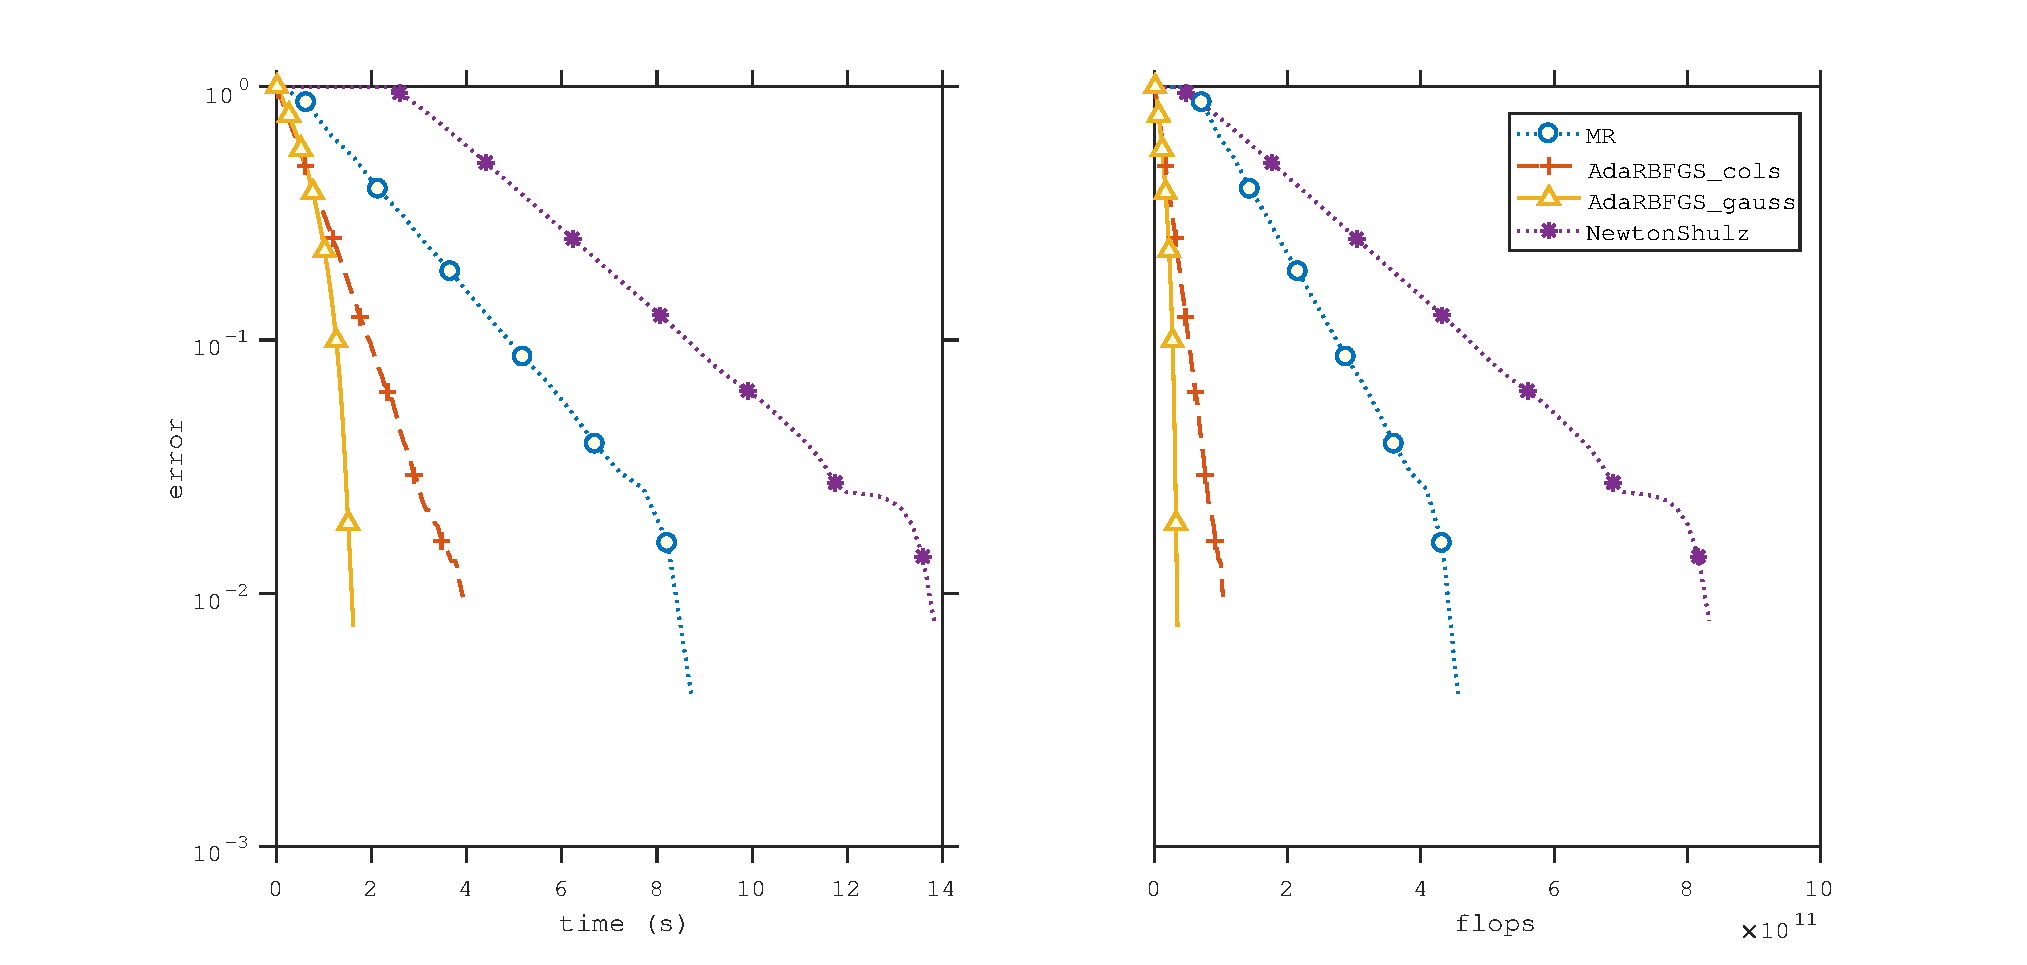
\includegraphics[height=0.7\columnwidth,width=1.1\columnwidth]{benchmark.eps}
  
  \vspace{-2mm}
  \caption{Empirical comparison of Ada-RBFGS variants against two standard methods for matrix inversion (Minimal residual and Newton-Schulz) for a $1000\times1000$ symmetric matrix.\label{fig:comparison}}  
  
\end{figure}

\section{Properties of RBFGS}\label{sect:propertiesRBFGS}
In this section we outline the main properties (as derived in \cite{Gower1}) that are useful to our analysis for the rate. A part from the rate analysis, the update rule for the $X_k$ iterates is the reason why adaRBFGS can be used as part of unconstrained convex function minimization methods and obtain known results in BFGS literature (as outlined in \ref{sect:primitive}). So, even if the expression for the update below does not seem to be very insightful, it is at the core of the properties we mention here.

\subsection{The update rule}
The update expression can be obtained from the constrain-and-approximate point of view (Section \ref{sect:framework}) by replacing the constraints in the objective and enforcing symmetry with an additional constraint (detailed derivation in \cite{Gower1}). We then obtain:
\begin{align}\label{eq:updaterule}
	&X_{k+1}=\\ \nonumber
    	&S(S^TAS)^{-1}S^T\\ \nonumber
	    &+ (I-S(S^TAS)^{-1}S^TA)X_k(I-AS(S^TAS)^{-1}S^T) \nonumber
\end{align}

One can see from equation \ref{eq:updaterule} that the update preservers symmetry and positive definitiveness (factorize $X_k$ and its left/right factors are symmetric, see \cite{Gower1} for a full proof). These two latter properties are important since we guarantee all iterates are non-singular, and symmetry is required in the results we use in Sections \ref{sect:convergence} and \ref{sect:sketchdim} (analysis of convergence and dependence of sketch dimension). Furthermore, this form also makes possible the Cholesky factorization and thus factored update derived in \cite{Gratton}.

\subsection{One-step progress and complete discrete sampling}
The starting point for an analysis of convergence is Thm. 6.2 in \cite{Gower1} (for which the one-step version is Thm.\ref{thm:onestep}). Then, an important question is: what conditions should random sketch matrix can satisfy in order to get a result like Thm. 6.2 in \cite{Gower1}. Actually, in order to have such a result the adaptive setting, the authors give a characterization for the support $\mathcal{S}$ where the $S_i$ (sketch matrices) are sampled from. Let $S=S_i\in R^{n\times q_i}$ with probability $p_i>0$ for $i \in [r]$ where $S_i$ has full column rank. And $S$ is defined as a complete discrete sampling when $\mathcal{S}=[S_1\ldots S_r]\in R^{n\times n}$ has full row rank.\\
Now, under the condition that the matrix we sample at each iteration is a complete discrete sampling we have:
\begin{customthm}{9.1}[Gower et al. 2016]\label{thm:onestep}
After one step of AdaRBFGS method we have\\
\\
$\E\Big[\norm{X_{k+1}-A^{-1}}^2_{F(A)}|X_k\Big] \leq \rho _k\norm{X_k-A^{-1}}^2_{F(A)}$
\end{customthm}
where $1-\rho_k=\lambda_{\text{min}}(A^{-1/2}\E\big[Z|X_k\big]A^{-1/2})$.\\
Given that the rate $\rho_k$ does not have an immediate interpretation, the authors in \cite{Gower1} propose a \textit{convenient sampling} of the form $p_i=\frac{Tr(S_i^TAS_i)}{Tr(S^TAS)}$ which yields the following upper bound $\rho_k \leq 1-\frac{\lambda_{\text{min}}(AX_k)}{Tr(AX_k)}$.\\
Note that such bound depends on the spectrum of $A$ preconditioned by $X_k$. Using the same form, $A$ preconditioned with $X_k$, we obtain in Section \ref{sect:results} a tighter upper bound for the rate and even a lower bound.


\section{Results}\label{sect:results}
\subsection{Interlacing spectrum}\label{sect:interlacing}
As mentioned in Section \ref{sect:propertiesRBFGS}, equation \ref{eq:updaterule} has some important consequences, among these is the interlacing spectrum (often known as Cauchy's interlacing spectrum theorem). Such update rule is a known result in the BFGS literature and can be derived under different circumstances. One such example comes from the equivalent formulation given by conjugate gradient with exact line search (as shown in \cite{Nazareth}). Moreover, a simple corollary of the interlacing spectrum is that the condition number is non-increasing (we use such consequence in the derivation of our proposed convenient sampling in Section \ref{sect:convsampling}) is a result independently found by Fletcher in \cite{Fletcher}.
Next, we state the interlacing spectrum theorem as applied to our setting.

\begin{customthm}{2.3}[Non-expansiveness Gratton 2011]\label{thm:interlacing}
Let $\sigma_1,\ldots\sigma_n$ real positive be the eigenvalues of $AX_{k}$ arranged in non-decreasing order. Then, the eigenvalues $\mu_1,\ldots,\mu_n$ of $AX_{k+1}$ can be arranged so that\\
\vspace{6mm}
$\left\{
    	\begin{array}{ll}
        	\sigma_j\leq\mu_j\leq\sigma_{j+q}\text{  for } j \in \{1,\ldots,n-q\}\\ 
            \mu_j=1 \text{                           for } j \in\{n-q+1,\ldots,n\}\\
        \end{array}                 
    \right.$
\end{customthm}
\vspace{-5mm}
It was first observed that adaRBFGS satisfies the interlacing spectrum property by Stich et al. in \cite{Stich1}. The proof is the same as that in \cite{Gratton} where the theorem we present is derived in a slightly different setting, namely, limited-memory preconditioners for least-squares problems. Note, however, that the proof basically relies on the form of update rule for $X_k$ (details in \cite{Gratton}) which can be factorized in two orthogonal components as presented in the following expression (part of the derivation in \cite{Gratton}).
\vspace{-7mm}
\begin{align}\label{eq:compression}
		A^{1/2}&X_{k+1}A^{1/2}
    	=\\ \nonumber
    	&\begin{bmatrix}
    		A^{1/2}W, & A^{1/2}\underline{W}
    	\end{bmatrix}
        \begin{bmatrix}
			I_q & 0\\
    		0 & V\Lambda V^T
		\end{bmatrix}
    	\begin{bmatrix}
    		W^TA^{1/2}\\
        	\underline{W}^TA^{1/2}
    	  \end{bmatrix} \nonumber
\end{align}
\vspace{-5mm}
\\
Where $W$ and $\underline{W}$ are $A$ orthogonal matrices, and $W=S(S^TAS)^{-1/2}$ (e.g. a term inside the factors that multiply $X_k$ when updating to $X_{k+1}$).
We observe in equation \ref{eq:compression} that first component $I_q$ has all 1 eigenvalues. Therefore, at each iteration (say the spectrum for $AX_{K+1}$) there are $q$ eigenvalues that are projected to 1 (where $q$ is the dimension of the sketch). Now, the second component $V\Lambda V^T=Q^TA^{1/2}X_kA^{1/2}Q$ (with $Q=A^{1/2}\underline{W}$) is a compression of the eigenvalues of the previous iterate (e.g. $AX_{k+1}$) which yields the interlacing property (see Corollary 4.3.16 in \cite{Horn}).\\
\begin{figure}[H]
  \centering
  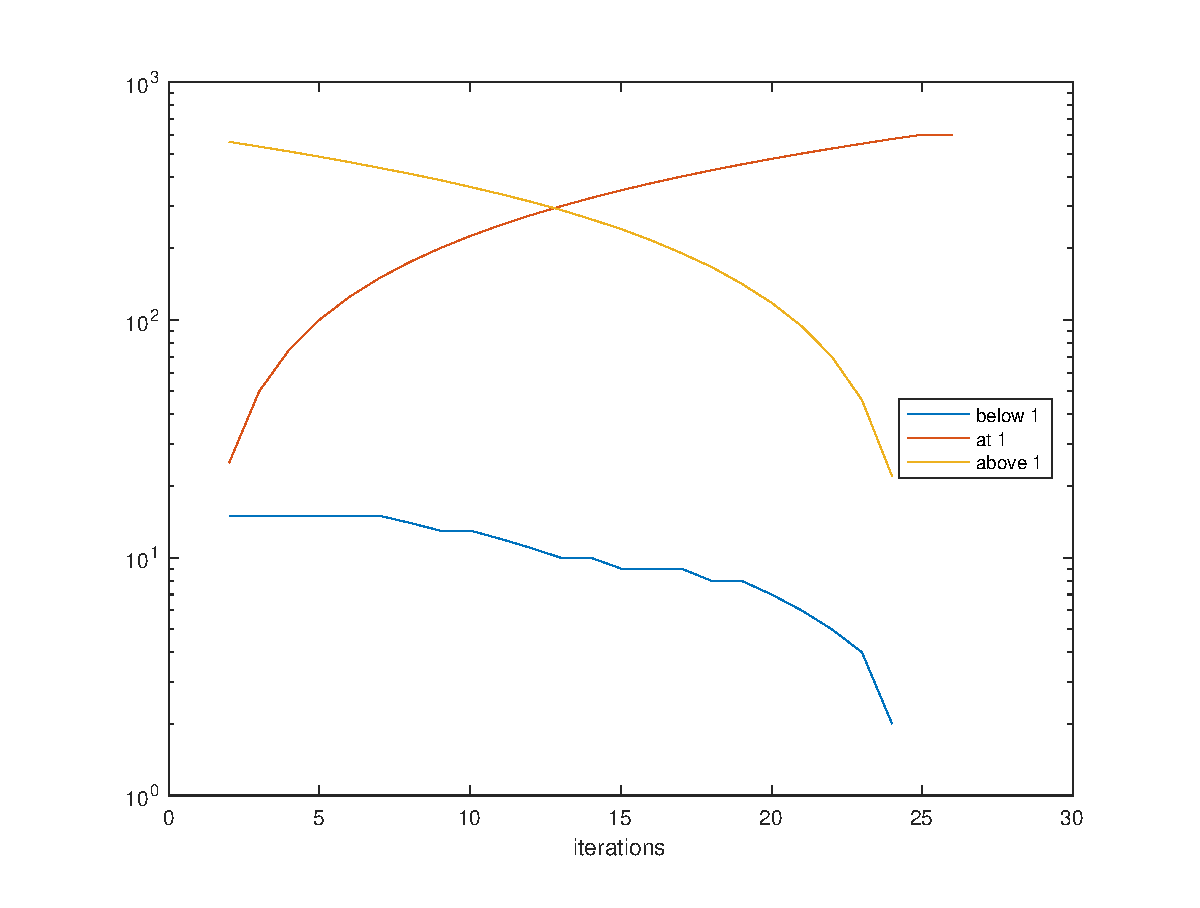
\includegraphics[height=0.7\columnwidth,width=1.0\columnwidth]{eigvalcountiter.eps}
  
  \vspace{-2mm}
  \caption{Eigenvalue count as a function of iterations for adaRBFGS (column variant). \label{fig:eigcount}}  
  
\end{figure}
A part from noticing that adaRBFGS matches the interlacing theorem conditions. We test experimentally whether an interlacing spectrum can be observed. The first such plot consists on the count of eigenvalues below, above and at 1 with thresholds defined by a tolerance band of $1e-2$ by default. Note in Fig. \ref{fig:eigcount} both eigenvalues above and below one decrease in a monotone manner while those at 1 increase strictly with the number of iterations which is evidence for the interlacing property. Although the spectrum for our input matrix $A$ always crosses $1$, we can always re-scale $A$ to have such a crossing spectrum (see \cite{Stich1,Gratton} without changing the system of equations to solve).\\
One important detail we observe in our experiments is the dependence of the number of iterations until convergence with respect to the initial maximum eigenvalue (e.g. $\lambda_{max}(A)$). We can further put in evidence the interlacing spectrum behavior by plotting the eigenvalue distribution for different thresholds of error convergence. For example, we show the histogram for adaRBFGS with a tolerance (relative error with respect to the initial error) of $1e^{-2}$ in Fig. \ref{fig:eighist2} and $1e^{-5}$ in Fig. \ref{fig:eighist5}. Observe that for a higher error threshold ($1e^{-2})$ the histogram has a tail to the right side which indicates ill conditioning of $AX_k$. And, as mentioned before, the number of iterations to 'loose' such tail is proportional to $\lambda_{max}(A)$. On the other side, for lower error threshold ($1e^{-5}$) we see that the eigenvalue distribution is centered around $1$ with little variation (e.g. $AX_k \approx I$).

\begin{figure}[H]
  \centering
  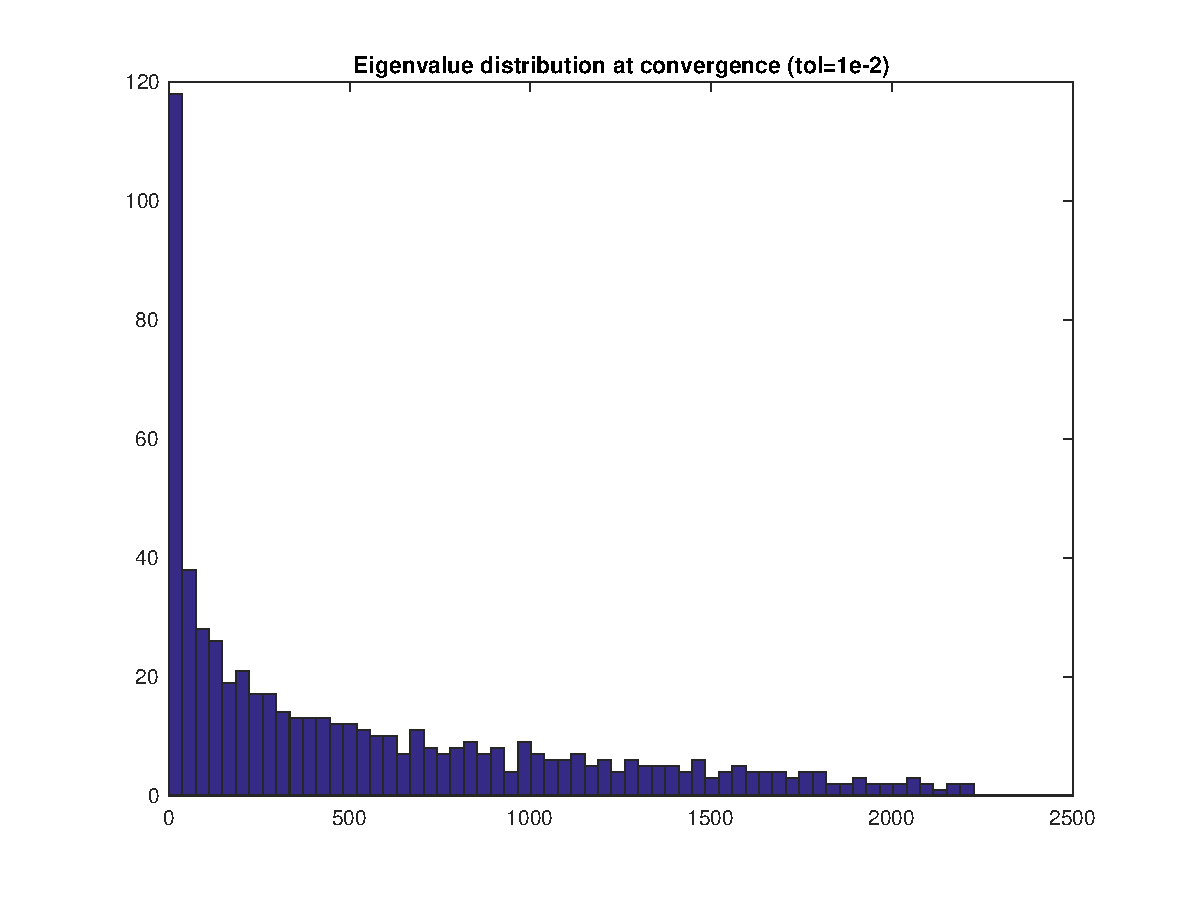
\includegraphics[height=0.7\columnwidth,width=1.0\columnwidth]{eigdisttol2.eps}
  
  \vspace{-2mm}
  \caption{Eigenvalue histogram after convergence, for the column variant of adaRBFGS, with tolerance $1e-2$ for the relative error. \label{fig:eighist2}}  
  
\end{figure}

The authors of adaRBFGS (c.f. \cite{Gower1}) make an intuitive guess on the asymptotic behavior of the spectrum. Namely, the idea of sampling from the Cholesky factor $L_k$ (see Section \ref{sect:adadef}) comes from the expectation of an optimized upper bound on the rate. Namely, Gower et al. make the conjecture that $\rho_k \leq 1- \frac{\lambda_{min}(AX_k)}{Tr(AX_k)}\rightarrow 1 - \frac{1}{n}.$ Therefore, the hope on the design of adaRBFGS is that $AX_k$ is well-conditioned in the limit. Yet, Gower et al. do not give the analysis on how or why this would happen and leave it for future research.\\
Once the interlacing property has been identified. A first observation is that the rate depends in the condition number (as it often does in BFGS or conjugate gradient methods) one sees that Thm.\ref{thm:interlacing} implies that the matrix $AX_k$ gets better conditioned (e.g. smaller gap between largest and smallest eigenvalues) and we would thus hope to converge to $X_k=A^{-1}$ (as $AX_k\approx I$).
\begin{figure}[H]
  \centering
  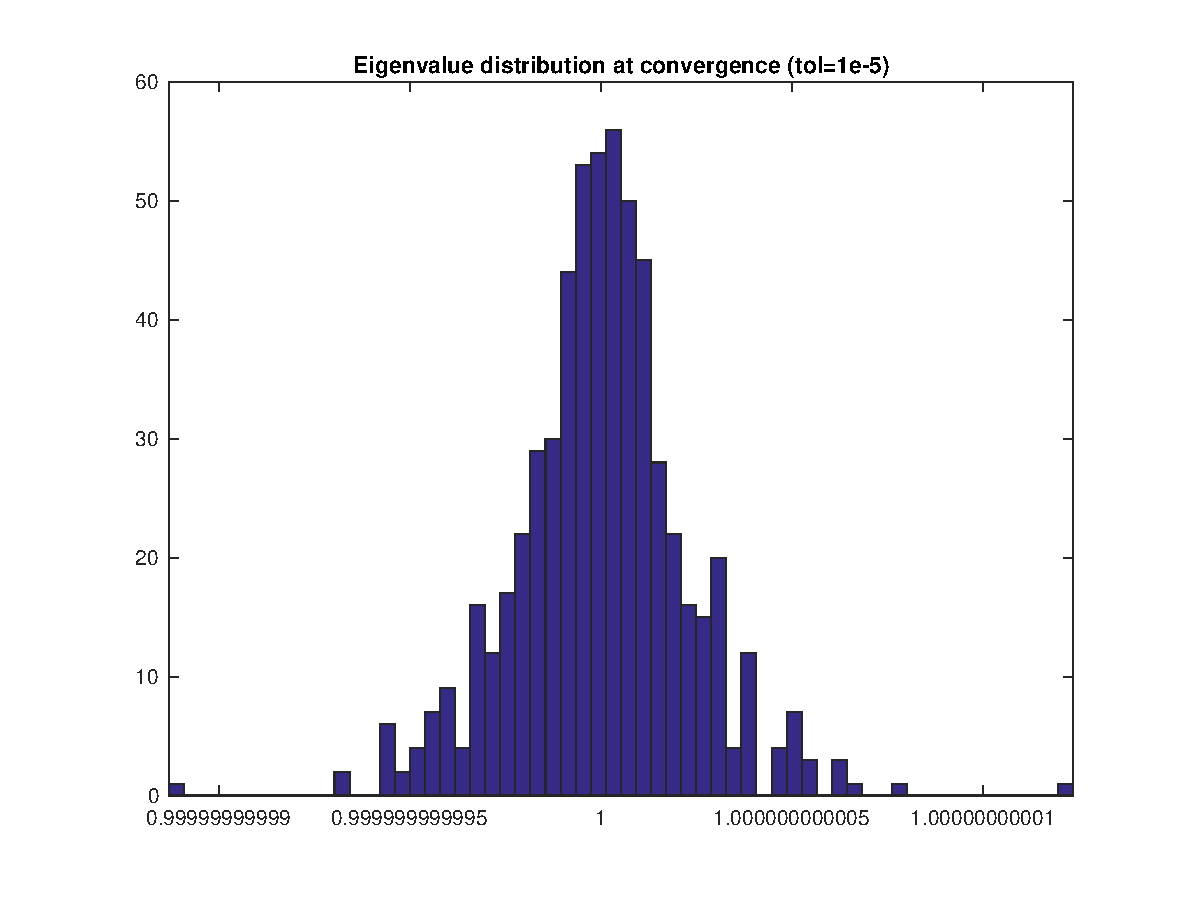
\includegraphics[height=0.7\columnwidth,width=1.0\columnwidth]{eigditstol5.eps}
  
  \vspace{-2mm}
  \caption{Eigenvalue histogram after convergence, for the column variant of adaRBFGS, with tolerance $1e-5$ for the relative error. \label{fig:eighist5}}  
  
\end{figure}

We conclude this section by exploring the interlacing spectrum property in the adaRBFGS gauss variant in Fig. \ref{fig:eigcountgauss}. We note that we have have a similar behavior as that for the spectrum of the column variant. However, note that those eigenvalues above $1$ get projected to $1$ at a much lower rate as in the column variant case. This experiment gives us some intuition in that $AX_k$ also gets better conditioned for the gaussian variant, which also hints why adaRBFGS in general has great performance against baselines in Fig. \ref{fig:comparison}. However, the results we present in Sections \ref{sect:adaptive rate} and \ref{sect:convsampling} have only been derived for the column variant. Hence, a theoretical analysis for gaussian or other adaptive distributions is left open for extension in future research.

\begin{figure}[H]
  \centering
  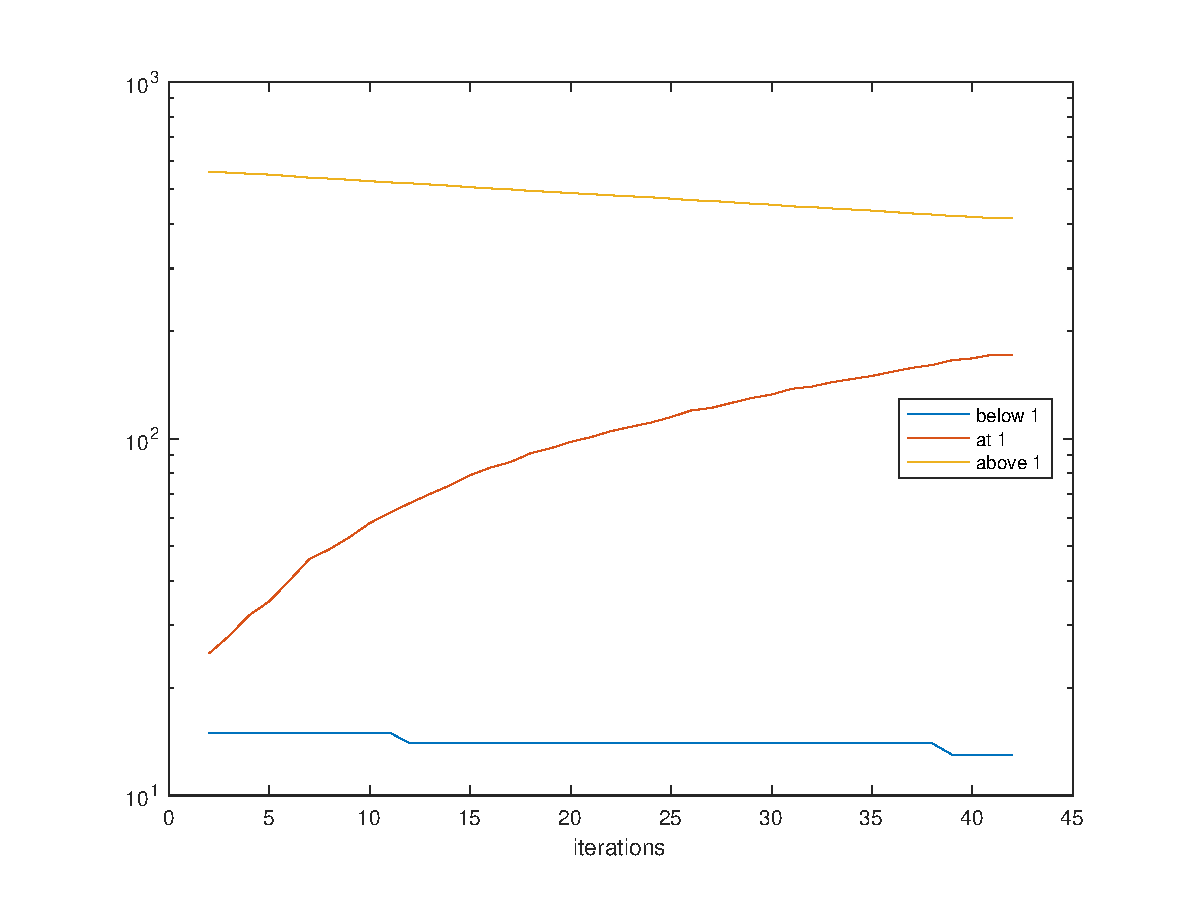
\includegraphics[height=0.7\columnwidth,width=1.0\columnwidth]{eigcountiter_gauss.eps}
  
  \vspace{-2mm}
  \caption{Eigenvalue count as a function of iterations for adaRBFGS for the gaussian variant. \label{fig:eigcountgauss}}  
  
\end{figure}

\subsection{Lower bound on adaptive rate}\label{sect:adaptive rate}
From Thm. \ref{thm:interlacing}, we have derived the following lower bound $\rho_k \geq 1-\frac{tr(D^2)}{tr(A^{-1/2}(L_k^T)^{-1}(L_k)^{-1}A^{-1/2})}=\rho_{lower}$. Where $D=Diag(\sqrt{p_1}(S_1^TAS_1)^{-1/2},\ldots,\sqrt{p_r}(S_r^TAS_r)^{-1/2})$. This comes, in fact, from a corollary of the interlace theorem for symmetric matrices as derived in \cite{J Tao,Fang} : $\lambda_{min}(A)tr(B)\leq tr(AB)$ for $A,B$ real symmetric and positive semi definite. Observe $\rho_{lower}$ for both adaRBFGS variants in Figures \ref{fig:ratemax} and \ref{fig:ratetr}. Note that this lower bound bound is especially useful for experiments using the (convenient) sampling strategy proposed in \cite{Gower1} (e.g. $p_i=\frac{tr(S_i^TAS_i)}{tr(\mathcal{S}^TA\mathcal{S})}$) as the upper bound ($\rho_{upper}$) is rather loose near convergence (as seen in Fig. \ref{fig:ratetr}). Thus $\rho_{upper}$ is not really a good indicator of the potential performance of the true rate (it is almost $2$ orders of magnitude off the true rate). Hence the lower bound, in this case, is a better indicator of the potential performance of the true rate.\\
Finally, we mention that we have also tried another rate lower bound which is a direct consequence of the interlacing theorem (see \cite{J Tao}), namely Schur's theorem $diag(B) \prec \lambda(B)$ where $B$ is the matrix in the definition of $\rho_k$. However, such lower bound did not present a quantitative improvement in our experiments, so we keep the first one.

\begin{figure}[H]
  \centering
  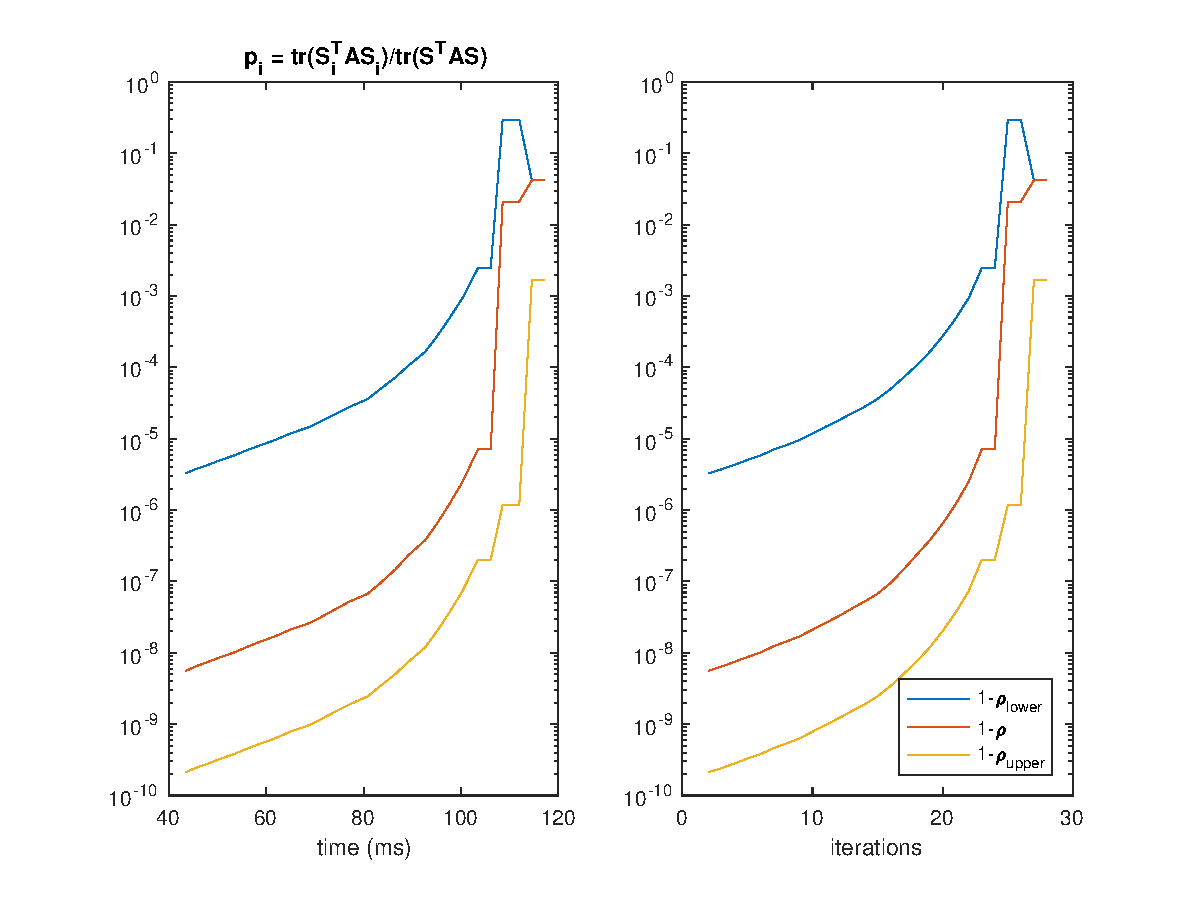
\includegraphics[height=0.7\columnwidth,width=1.1\columnwidth]{ratetr.eps}
  
  \vspace{-2mm}
  \caption{1 minus rate and respective lower/upper bounds for the column variant of adaRBFGS with the proposed convenient sampling $p_i$ of Gower et al. \cite{Gower1} \label{fig:ratetr}}  
  
\end{figure}

\subsection{A more concise convenient sampling and non-increasing upper bound}\label{sect:convsampling}
The reason why Gower et al. pick $p_i=\frac{tr(S_i^TAS_i)}{tr(\mathcal{S}^TA\mathcal{S})}$ as convenient sampling in \cite{Gower1} is that such sampling yields an optimal upper bound. Namely, $1-\frac{\lambda_{min}(AX_k)}{tr(AX_k)} \rightarrow 1-\frac{1}{n}$. We remark, however, two potential inefficiencies in this derivation. First, the upper bound $1-\frac{1}{n}$ simply corresponds to $AX_k\approx I$ (see Section \ref{sect:interlacing}) thus, we should be able to find $\rho_{upper}$ that converges to a perhaps simpler function of the spectrum of the identity matrix. Second, on the derivation for the rate upper bound in \cite{Gower1} (proof of Thm. 9.1) the sequence of inequalities can be optimized (e.g. we only use the first inequality of such proof) by setting $p_i=\frac{\lambda_{max}(S_i^TAS_i)}{\lambda_{max}(\mathcal{S}^TA\mathcal{S})}$ which yields as rate upper bound $\rho_{upper}=1-\kappa (AX_k)^{-1}=1-\frac{\lambda_{min}(AX_k)}{\lambda_{max}(AX_k)}\geq \rho_k$.\\
We can then outline the advantage of our proposed convenient sampling approach by the experiments in Figures \ref{fig:ratemax} and \ref{fig:ratetr}. First, note in those experiments that $\rho_{upper}$ for Gower's $p_i$ yields loose upper bounds. Hence a lower bound is useful to realize the potential value of the true rate as in Section \ref{sect:convsampling}. On the other hand, observe (Fig. \ref{fig:ratemax}) that our proposed $\rho_{upper}$ is much tighter (at all times) with respect to the true rate. In addition, note that the sampling we propose can actually make the true rate hit much lower values (in Fig.\ref{fig:ratemax} this corresponds to $1-\rho$ hitting 1) which is not the case for Gower's convenient sampling (Fig. \ref{fig:ratetr})\\
Moreover, the theoretical analysis is simpler and we can state the following result as a corollary from Thm. \ref{thm:interlacing}: $\frac{\lambda_{min}(AX_k)}{\lambda_{max}(AX_k)} \leq \frac{max\{1,\lambda_{min}(AX_{k+1})\}}{max\{1,\lambda_{max}(AX_{k+1})\}}$ which means that our proposed rate upper bound is non-increasing. Note that such concise conclusion is rather difficult if we work with $tr(AX_k)$ as it is done in \cite{Gower1}, and this is because not all eigenvalues are guaranteed to be above 1. Hence, in such scenario the interlacing theorem does not yield an immediate result with respect to the monotonicity of the rate upper bound.\\
\begin{figure}[H]
  \centering
  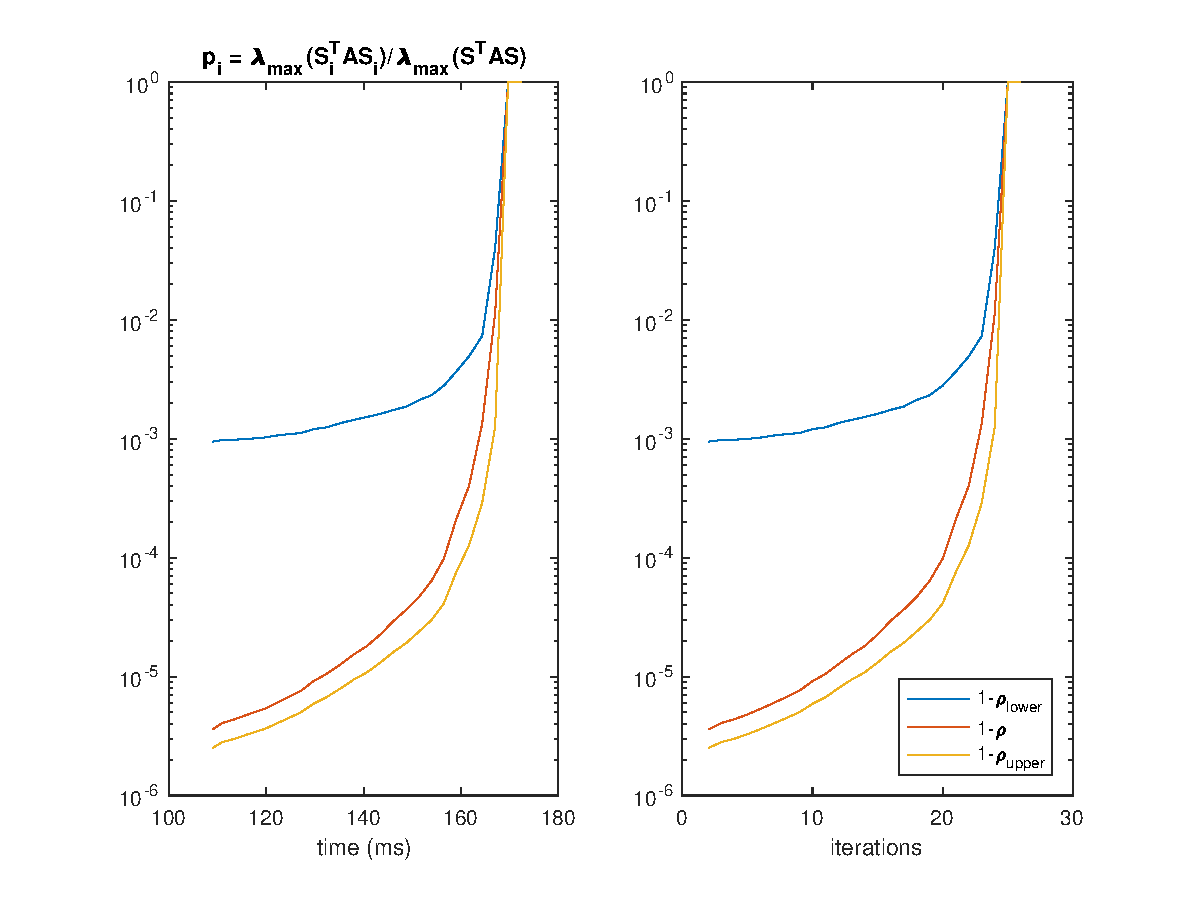
\includegraphics[height=0.7\columnwidth,width=1.1\columnwidth]{ratemax.eps}
  
  \vspace{-2mm}
  \caption{1 minus rate and respective lower/upper bounds for the column variant of adaRBFGS with our proposed convenient sampling $p_i$. \label{fig:ratemax}}  
  
\end{figure}
A non-increasing rate upper bound (as the one we propose) has an immediate consequences (as pointed out in \cite{Stich1}). First, the adaptive version of RBFGS (e.g. adaRBFGS) can only be better (in expectation) than the non-adaptive version. Namely, if $\lambda_{min}(A) \leq 1$ then $\prod_{i=0}^{k-1}\rho\prime_{i} \leq \rho\prime^{k}_0$ where $\rho\prime=\rho_{upper}$. To see this, simply set $\rho\prime_0$ as the rate of the non-adaptive RBFGS.
\subsection{Convergence}\label{sect:convergence}
As we saw in our experiments (and conjectured in \cite{Gower1}) the eigenvalues converge to a distribution centered at 1 and with very low variance.\\
We have found, in fact, that a good framework for studying such behavior is given by some well-known results from Random Matrix theory (which we borrow from \cite{Tao}).\\
In order to explain how can adaRBFGS make progress at each iteration we refer to the \textit{repulsive eigenvalues} property (Exercise 1.3.15 in \cite{Tao}). This is, actually, a direct consequence of the interlacing spectrum theorem. In additino and it reveals a fundamental relation between eigenvalues and how these change as we iterate. The property we present (repulsiveness of the spectrum) is in fact used to prove some of the main results in \cite{Tao} (see for example the Dyson Brownian motion characterization of the spectrum). We can state the repulsive eigenvalues property as follows. Let, $\lambda$ be an eigenvalue for $AX_{k}$ that is different from all eigenvalues for $AX_{k+1}$, we can write $(AX_{k})_{n,n}-\lambda = \sum_{j=1}^{n-1}\frac{|u_j(A_{k+1})^TX|}{\lambda_j(AX_{k+1})-\lambda}$. Where $u_j$ is the $j^{th}$ eigenvector and $X$ is a vector we cut from $AX_k$ to get to $AX_{k+1}$ as its minor (equivalent definition for compression in \cite{Horn}). Now, we see from the above formula that $\lambda$ is a rational function with removable poles at $\lambda_j(AX_{k+1}$. This means that as long as the update direction from $AX_k$ to $AX_{k+1}$ does not lead to an orthogonal eigenvector to $X$ then eigenvalues repel each other between iterations.\\
It turns out that there is a set of results in Random Matrix theory that characterize the distribution of eigenvalues and these stem from an interlacing spectrum. For this purpose, we work with the Empirical Spectrum Distribution (ESD). Namely, $\mu_{AX_k} = \frac{1}{n} \sum _{j=1}^{n} \delta_{\lambda_j(AX_k)}$. The main results that concern us from \cite{Tao} are those that involve the stability of the ESD and its asymptotic convergence properties.\\
A first result is the \textit{Stability of ESD laws with respect to small rank perturbation} for symmetric matrices (note that adaRBFGS is defined to minimize the rank of updates at each iteration). What this result says (applied to our setting) is that $\mu_{AX_{k+1}}$ converges almost surely to fixed $\mu$ which could prove convergence of adaRBFGS. Now, we do not have a explicit expression for $\mu$ in our setting because at the moment this theory is beyond the scope of this project. As an illustration we mention a generalization of the above result which is the Semicircular law (for sequences of Wigner matrices) which gives an explicit formula for $\mu$. While Wigner matrices are more of a theoretical construction (infinite matrices), there are some results in \cite{Tao} that make the connexion with finite i.i.d and non i.i.d matrices.\\
A second set of results from \cite{Tao} that are relevant to convergence of adaRBFGS are the (weak-strong) versions of the Bai-Yin theorem (c.f. Theorem 2.3.23 in \cite{Tao}). What is important, for us, about Bai-Yin theorems (applied to real symmetric matrix sequences) is that these show that the spectral radius ($\lambda_{max}$ in our setting) of $AX_k$ is asymptotically bounded by a constant (asymptotically almost surely). Then, the convergence of the ESD and Bai-Yin theorems altogether would imply that $AX_k$ is well conditioned asymptotically almost surely.

\begin{figure}[H]
  \centering
  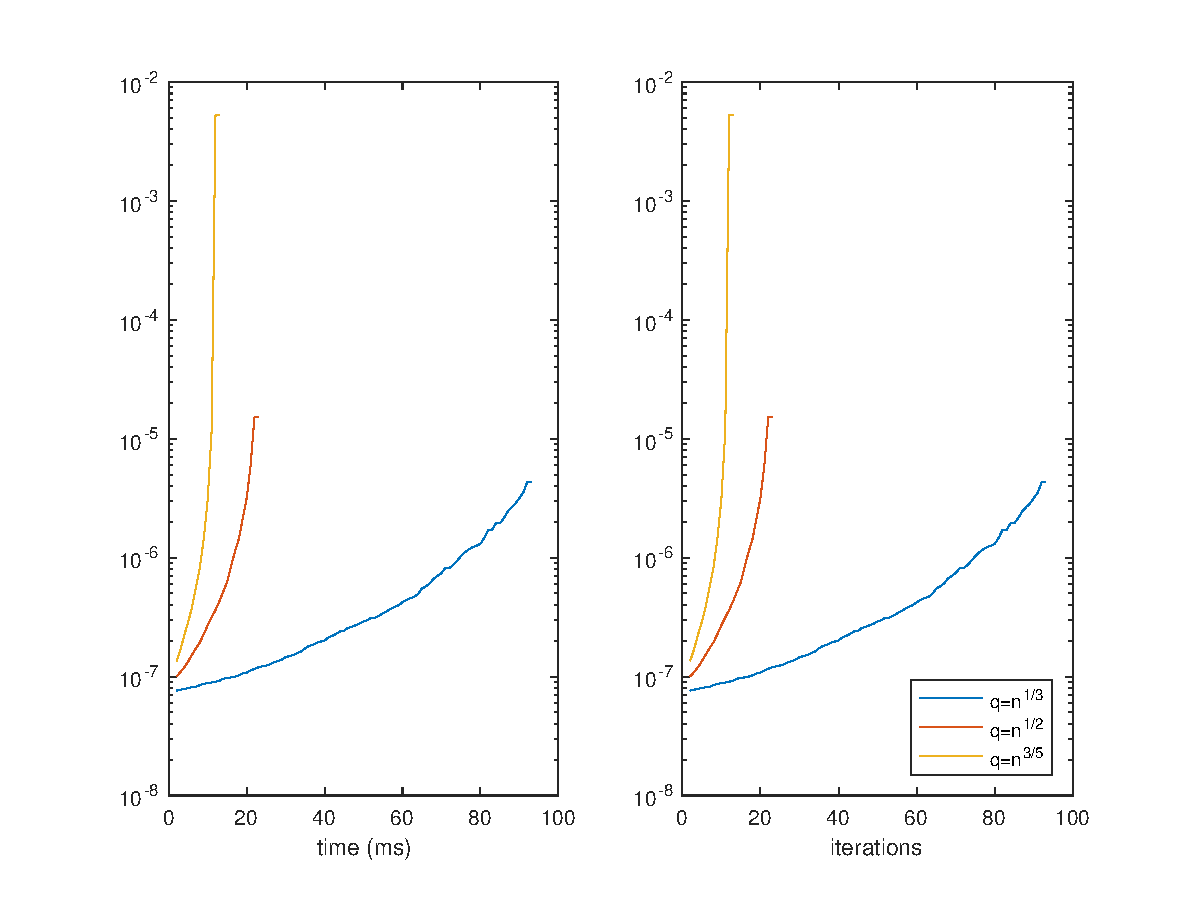
\includegraphics[height=0.7\columnwidth,width=1.1\columnwidth]{ratedim.eps}
  
  \vspace{-2mm}
  \caption{Rates for adaRBFGS (column variant) as a function of the dimension of the sketch (e.g. q). \label{fig:ratedim}}  
  
\end{figure}

\subsection{Dependence on sketch dimension}\label{sect:sketchdim}
Our last result concerns a particular behavior we have observed during the experiments which is the dependence of the number of iterations on the sketch dimension $q$. A first result in this direction is the lower bound presented in \cite{Gower1} for the non-adaptive RBFGS (constant rate), which is $1-\frac{\E[q]}{n}\leq \rho $. What the previous result implies that increasing the sketch dimension $q$ can only make the constant rate smaller. Nonetheless, there is a clear trade-off with respect to the complexity per iteration (floating point operations) which is dominated by a matrix inversion (see update rule in Section \ref{sect:rbfgs}) of order $q$ e.g. $O(q^{1/3})$. Now, we want to know how the sketch dimension depends on the rate for the adaptive setting (e.g. adaRBFGS). We observe in numerical experiments in Fig. \ref{fig:ratedim} that the $1-\rho_k$ (1 minus the true rate) can only converge faster. One can justify this observation with a result stemming (again) from Thm. \ref{thm:interlacing} which is a characterization of the stability of the ESD (which comes from 2.4.1 in \cite{Tao}). Stability of the ESD can be described as $\frac{k+1}{k}q^c\mu_{AX_k}([-\infty,x])-\frac{q^c}{k} \leq \mu_{AX_{k+1}}([-\infty,x])\leq \frac{k+1}{k}q^c\mu_{AX_k}([-\infty,x])$ with $0<c<1$. We observe from this last result that when $q$ is large then the ESD can change quite a lot from one iteration to the other. However, for $q$ very small the ESD is stable (e.g. changes very little) in one iteration. In this case having an unstable ESD (large $q$) is beneficial when we have large $\lambda_{max}(A)$ as we want to eliminate, as quickly as possible, the tail  (as seen in Section \ref{sect:rbfgs}) composed of large eigenvalues that result in ill-conditioning for $AX_k$. In such scenario, a stable distribution progression could take quite long to eliminate the tail (as we confirm in Fig. \ref{fig:ratedim}).
\section{Conclusion}\label{sect:conclusion}
In this project we have analyzed the rate for adaRBFGS which is new promising method that can be used as a primitive for first and second order methods. In the process we have surveyed related literature that serves as basis for adaRBFGS and pointed out some additional results that are useful for a finer grained analysis of the algorithm's rate (which were apparently unnoticed by the authors in \cite{Gower1}). A first such result and the starting point of our analysis is the interlacing spectrum theorem (c.f. \ref{sect:interlacing}). Such property suggests that the spectrum of $AX_k$ shrinks as we iterate, and that eigenvalues accumulate at 1 (which was conjectured in \cite{Gower1}). In addition, we propose a different convenient sampling strategy (to sample sketch matrices for adaRBFGS) for which we get (c.f. \ref{sect:convsampling}) a simpler theoretical analysis for the rate (using the interlacing theorem). We observed as consequence of this proposed sampling strategy that both a lower and upper bound we derived look much tighter (experimentally) than the previously known bounds in \cite{Gower1}. Then, as direct consequence of the form of our upper bound and the interlacing theorem we saw that the rate upper bound is non-increasing and that adaRBFGS outperforms RBFGS (non adaptive version). We point out, however, that we observed experimentally that the true rate $\rho_k$ is also non-increasing. However, the proof of such result is not as straightforward. In fact, if this result is of interest for future result we suggest looking at the relation between subsequent column matrices of $L_k$ and $L_{k+1}$, namely $S_i^k$ and $S_i^{k+1}$. It is not hard to see that (from the Courant-Fisher characterization of eigenvalues) that if one could prove either $S_i^k \succ S_i^{k+1}$ (or the opposite) at each iteration, then $\rho_k$ is non-increasing. Moreover, $\rho_k$ for adaRBFGS seems to have better convergence behavior in our experiments. With these results in mind, we embarked on the analysis of convergence for the rate. For this purpose we borrowed results from random matrix theory. This is because such theory has a rich description on the asymptotic and stochastic properties for the spectrum of sequence of matrices such as those we generate for adaRBFGS. Namely, these results describe stability and convergence modes for the Empirical Spectrum Distribution (ESD), that gives us additional theoretical justification on the experimental results (centered distributions around 1) we see. While the results we used are rather general, there is potentially room for specialization as the ones existing for other type of matrices (such as the semi-circle law in \cite{Tao}). Lastly, we used the stability of the ESD to investigate the relation between the sketch dimension $q$ and the true adaRBFGS rate. While there is a result for the non-adaptive version (Theorem 6.1 in \cite{Gower1}) there was no obvious way to extend this to adaRBFGS which is why we investigated this behavior. A next step would be to make explicit the trade-off between the number of iterations and flops per iteration in terms of $q$ and $n$ (number of dimensions). Such question is appealing as it would answer a very practical question for the use of adaRBFGS: how to choose $q$ that is most efficient for my problem?. Lastly, we mention an interesting direction for future research. This consists of going beyond proving that the rate (or its upper bound) are non-increasing (as proved in Section \ref{sect:convsampling}) and finding the sequence of decrement ratios between subsequent rates. Such a result is plausible as the convergence time depends mainly on $\lambda_{max}(AX_k)$ and a set of results for bounding the spectral radius have been derived using related to the interlacing spectrum (c.f. \cite{Mercer,Horne}).



\bibliographystyle{IEEEtran}
%\bibliography{literature}
\begin{thebibliography}{1}

\bibitem{Gower1}
\textit{Randomized quasi-Newton updates are linearly convergent matrix inversion algorithms.}
R.M.Gower and P.Richtarik. arXiv:1602.01768, 2016.

\bibitem{Gower2}
\textit{Randomized iterative methods for linear systems.} R.M. Gower and P. Richtarik. SIAM Journal on Matrix Analysis and Applications 36.4, pp. 1660-1690, 2015.
\bibitem{Gower3}
\textit{Stochastic Block BFGS: Squeezing More Curvature our of Data.} R.M. Gower, D. Goldfarb and P. Richtarik. Proceedings of The 33rd International Conference on Machine Learning, PMLR 48:1869-1878, 2016.
\bibitem{Gowercode}
\textit{A suite of randomized methods for inverting positive definite matrices implemented in MATLAB.} Robert M Gower. \url{http://www.maths.ed.ac.uk/~prichtar/i_software.html}.

\bibitem{Gratton}
\textit{On a class of limited memory preconditioners for large-scale nonlinear least-squares problems.} SIAM Journal on Optimization 21.3, pp. 912-935, 2011.

\bibitem{Horn}
\textit{Matrix Analysis.} R.A. Horn and C.R. Johnson. Cambridge University Press, Cambridge, England, 1999.
\bibitem{Nazareth}
\textit{A relationship between the BFGS and conjugate gradient algorithms and its implications for new algorithms.} L. Nazareth. SIAM Journal on Numerical Analysis, 16:794-800, 1979.

\bibitem{Fletcher}
\textit{A new approach to variable metric algorithms.} R. Fletcher. Computer Journal, 13:317-322, 1970.

\bibitem{Tao}
\textit{Topics in Random Matrix Theory.} Terrence Tao. Graduate Studies in Mathematics, Volume 132. American Mathematical Society, 2012.

\bibitem{Fang}
\textit{Eigenvalue Inequalities for Matrix Product.} Fuzhen Zhang and Qingling Zhang. IEEE Transactions on Automatic Control, 2006.

\bibitem{J Tao}
\textit{The Cauchy interlacing theorem in simple Euclidean Jordan algebras and some consequences.}
M. Seetharama Gowda and J. Tao. Linear and Multilinear Algebra, 16:41, 2009.

\bibitem{Mercer}
\textit{Cauchy's interlace theorem and lower bounds for the spectral radius.} A.Mcd. Mercer and Peter R. Mercer. International Journal of mathematics and Mathematical Sciences. Vol. 23, Issue 8, pp. 563-566, 2000.

\bibitem{Horne}
\textit{Lower bounds for the spectral radius of a matrix.} Bill G. Horne. NECI Technical Report 95-14, NEC Research Institute, 1995.

\bibitem{Stich1}
Sebastian U. Stich.
\textit{Complexity of Adaptive Randomized BFGS for Matrix Inversion.}
Preprint, 2016.

\bibitem{Stich2}
\textit{Variable metric random pursuit.} S. U. Stich, C.L. Muller, and B.Gartner. Mathematical
Programming 156.1 (2015), pp. 549-579.

\bibitem{Leventhal}
\textit{Randomized Hessian estimation and directional search.} D.Leventhal and A.Lewis. Optimization 60.3(2011), pp. 329-345.

\bibitem{variancereduct}
\textit{Accelerating stochastic gradient descent using predictive variance reduction.}Rie Johnson, Tong Zhang.Advances in Neural Information Processing Systems. pp. 315-323, 2013.

\end{thebibliography}

\end{document}
